\documentclass{article}%
\usepackage[T1]{fontenc}%
\usepackage[utf8]{inputenc}%
\usepackage{lmodern}%
\usepackage{textcomp}%
\usepackage{lastpage}%
\usepackage{parskip}%
\usepackage[top=1.2in,bottom=1in,left=0.6in,right=0.6in,headsep=0.8in]{geometry}%
\usepackage{amsmath}%
\usepackage{graphicx}%
\usepackage{needspace}%
\usepackage{color}%
\usepackage{longtable}%
\usepackage{multirow}%
\usepackage[table]{xcolor}%
\usepackage{fancyhdr}%
\usepackage{tabularx}%
%
\definecolor{OsdagGreen}{HTML}{D5DF93}%
\fancypagestyle{header}{ 
\renewcommand{\headrulewidth}{0pt}%
\renewcommand{\footrulewidth}{0pt}%
\fancyhead{ 
}%
\fancyfoot{ 
}%
\fancyhead[C]{ 
\renewcommand{\arraystretch}{1.2}%
\begin{tabularx}{\textwidth}{|l|p{6cm}|l|X|}%
\hline%
\rowcolor{OsdagGreen}%
Company Name&fhned&Project Title&\\%
\hline%
\rowcolor{OsdagGreen}%
Group/Team Name&&Subtitle&\\%
\hline%
\rowcolor{OsdagGreen}%
Designer&&Job Number&\\%
\hline%
\rowcolor{OsdagGreen}%
Date&29 /04 /2020&Client&\\%
\hline%
\end{tabularx}
}%
\fancyfoot[R]{ 
Page \thepage\ of \pageref{LastPage}
}
}%
%
\begin{document}%
\normalsize%
\pagestyle{header}%
\section{Input Parameters}%
\label{sec:InputParameters}%
\renewcommand{\arraystretch}{1.2}%
\begin{longtable}{|p{5cm}|p{2cm}|p{2cm}|p{2cm}|p{5cm}|}%
\hline%
\hline%
\multicolumn{3}{|c|}{Module}&\multicolumn{2}{|c|}{Tension Members Bolted Design}\\%
\hline%
\hline%
\multicolumn{3}{|c|}{Axial (kN) *}&\multicolumn{2}{|c|}{400.0}\\%
\hline%
\hline%
\multicolumn{3}{|c|}{Length(mm) *}&\multicolumn{2}{|c|}{2000.0}\\%
\hline%
\hline%
\multicolumn{5}{|c|}{\textbf{Section}}\\%
\hline%
\hline%
\multirow{15}{*}{\includegraphics[width=5cm,height=5cm]{"E:/workspace/Osdag3/ResourceFiles/images/Unequal".png}}&\multicolumn{2}{|c|}{Section Size*}&\multicolumn{2}{|c|}{('100 65 X 6', 'Back to Back Angles')}\\%
\cline{2%
-%
5}%
&\multicolumn{2}{|c|}{Material *}&\multicolumn{2}{|c|}{E 250 (Fe 410 W)A}\\%
\cline{2%
-%
5}%
&\multicolumn{2}{|c|}{Ultimate strength, fu (MPa)}&\multicolumn{2}{|c|}{410}\\%
\cline{2%
-%
5}%
&\multicolumn{2}{|c|}{Yield Strength , fy (MPa)}&\multicolumn{2}{|c|}{230}\\%
\cline{2%
-%
5}%
&Mass&7.5&Iu(mm4)&978000.0\\%
\cline{2%
-%
5}%
&Area(mm2) {-} A&958.0&Iv(mm4)&335000.0\\%
\cline{2%
-%
5}%
&A(mm)&100.0&rz(mm)&32.1\\%
\cline{2%
-%
5}%
&B(mm)&65.0&ry(mm)&18.5\\%
\cline{2%
-%
5}%
&t(mm)&0.0&ru(mm)&32.0\\%
\cline{2%
-%
5}%
&R1(mm)&8.0&rv(mm)&18.7\\%
\cline{2%
-%
5}%
&R2(mm)&0.0&Zz(mm3)&14500.0\\%
\cline{2%
-%
5}%
&Cy(mm)&15.4&Zy(mm3)&6600.0\\%
\cline{2%
-%
5}%
&Cz(mm)&32.0&Zpz(mm3)&26400.0\\%
\cline{2%
-%
5}%
&Iz(mm4)&980000.0&Zpy(mm3)&6600.0\\%
\cline{2%
-%
5}%
&Iy(mm4)&330000.0&&\\%
\cline{2%
-%
5}%
\hline%
\multicolumn{5}{|c|}{\textbf{Bolt Details}}\\%
\hline%
\hline%
\multicolumn{3}{|c|}{Diameter(mm)*}&\multicolumn{2}{|c|}{{[}12.0, 16.0, 20.0, 24.0, 30.0, 36.0{]}}\\%
\hline%
\hline%
\multicolumn{3}{|c|}{Grade *}&\multicolumn{2}{|c|}{{[}3.6, 4.6, 4.8, 5.6, 5.8, 6.8, 8.8, 9.8, 10.9, 12.9{]}}\\%
\hline%
\hline%
\multicolumn{3}{|c|}{Type *}&\multicolumn{2}{|c|}{Bearing Bolt}\\%
\hline%
\hline%
\multicolumn{3}{|c|}{Bolt hole type}&\multicolumn{2}{|c|}{Standard}\\%
\hline%
\hline%
\multicolumn{3}{|c|}{Bolt Ultimate Strength (N/mm2)}&\multicolumn{2}{|c|}{500.0}\\%
\hline%
\hline%
\multicolumn{3}{|c|}{Bolt Yield Strength (N/mm2)}&\multicolumn{2}{|c|}{300.0}\\%
\hline%
\hline%
\multicolumn{3}{|c|}{Slip factor (µ\_f)}&\multicolumn{2}{|c|}{0.3}\\%
\hline%
\hline%
\multicolumn{3}{|c|}{Type of edges}&\multicolumn{2}{|c|}{a {-} Sheared or hand flame cut}\\%
\hline%
\hline%
\multicolumn{3}{|c|}{Gap between beam and <br>support (mm)}&\multicolumn{2}{|c|}{0.0}\\%
\hline%
\hline%
\multicolumn{3}{|c|}{Are the members exposed to <br>corrosive influences}&\multicolumn{2}{|c|}{False}\\%
\hline%
\end{longtable}

%
\Needspace{10\baselineskip}%
\newpage%
\section{Design Checks}%
\label{sec:DesignChecks}%
\subsection{Member Checks}%
\label{subsec:MemberChecks}%
\renewcommand{\arraystretch}{1.2}%
\begin{longtable}{|p{3cm}|p{5cm}|p{7cm}|p{1cm}|}%
\hline%
\rowcolor{OsdagGreen}%
Check&Required&Provided&Remarks\\%
\hline%
\endhead%
\hline%
Tension Yielding Capacity (kN)&&$\begin{aligned}T_{dg} &= \frac{A_g ~ f_y}{\gamma_{m0}}\\ &= \frac{2*958.0*230}{1.1}\\ &= 400.62\end{aligned}$&\\%
\hline%
Tension Rupture Capacity(kN)&&$\begin{aligned}\beta &= 1.4 - 0.076*\frac{w}{t}*\frac{f_{y}}{f_{u}}*\frac{b_s}{L_c}\\ &\leq\frac{0.9*f_{u}*\gamma_{m0}}{f_{y}*\gamma_{m1}} \geq 0.7 \\ &= 1.4 - 0.076*\frac{65.0}{6.0}*\frac{230}{410}*\frac{116.0}{180 }\\ &\leq\frac{0.9* 410*1.1}{230*1.25} \geq 0.7 \\ &= 1.07\\ T_{dn} &= 2*(\frac{0.9*A_{nc}*f_{u}}{\gamma_{m1}} + \frac{\beta * A_{go} * f_{y}}{\gamma_{m0}})\\ &= 2*(\frac{0.9* 432.0*410}{1.25} + \frac{1.07*390.0*230}{1.1})\\ &= 429.56\end{aligned}$&\\%
\hline%
Block Shear Capacity (KN)&&$\begin{aligned}T_{db1} &= \frac{A_{vg} f_{y}}{\sqrt{3} \gamma_{m0}} + \frac{0.9 A_{tn} f_{u}}{\gamma_{m1}}\\ T_{db2} &= \frac{0.9*A_{vn} f_{u}}{\sqrt{3} \gamma_{m1}} + \frac{A_{tg} f_{y}}{\gamma_{m0}}\\ T_{db} &= min(T_{db1}, T_{db2})= 400.36\end{aligned}$&\\%
\hline%
Tension Capacity (kN)&&$\begin{aligned} T_d &= Min(T_{dg},T_{dn},T_{db})\\ &= Min(400.62,429.56,400.36)\\ &=400.36\end{aligned}$&Pass\\%
\hline%
Slenderness&$\begin{aligned}\frac{K * L}{r} &\leq 400\end{aligned}$&$\begin{aligned}\frac{K * L}{r} &= \frac{1*2000.0}{34.11}\\ &= 58.64\end{aligned}$&\\%
\hline%
Efficiency&$\begin{aligned} Efficiency &\leq 1 \end{aligned}$&$\begin{aligned} Efficiency &= \frac{F}{Td}&=\frac{400.0}{400.36}\\ &= 1.0\end{aligned}$&\\%
\hline%
\end{longtable}

%
\newpage%
\subsection{Bolt Checks}%
\label{subsec:BoltChecks}%
\renewcommand{\arraystretch}{1.2}%
\begin{longtable}{|p{3cm}|p{5cm}|p{7cm}|p{1cm}|}%
\hline%
\rowcolor{OsdagGreen}%
Check&Required&Provided&Remarks\\%
\hline%
\endhead%
\hline%
Diameter(d) (mm)&Bolt Quantity Optimisation&20.0&\\%
\hline%
Grade&Bolt Grade Optimisation&5.6&\\%
\hline%
Bolt Hole Diameter(d0) (mm)& &22.0&\\%
\hline%
Shear Capacity (kN)&&$\begin{aligned}V_{dsb} &= \frac{f_ub ~n_n~ A_{nb}}{\sqrt{3} ~\gamma_{mb}}\\ &= \frac{500.0*2*245}{\sqrt{3}~*~1.25}\\ &= 113.16\end{aligned}$&\\%
\hline%
Bearing Capacity (kN)&&$\begin{aligned}V_{dpb} &= \frac{2.5~ k_b~ d~ t~ f_u}{\gamma_{mb}}\\ &= \frac{2.5~*0.61*20.0*12.0*410}{1.25}\\ &=120.05\end{aligned}$&\\%
\hline%
Capacity (KN)&&$\begin{aligned}V_{db} &= min~ (V_{dsb}, V_{dpb})\\ &= min~ (113.16,120.05)\\ &=113.16\end{aligned}$&\\%
\hline%
No of Bolts (n)&$\begin{aligned}R_{u} &= \sqrt{V_u^2+A_u^2}\\ n_{trial} &= R_u/ V_{bolt}\\ R_{u} &= \frac{\sqrt{0.0^2+400.0^2}}{113.16}\\ &=4\end{aligned}$&4&\\%
\hline%
No of Columns (nc)&&4&\\%
\hline%
No of Rows (nr)&&1&\\%
\hline%
Min. Pitch (mm)&$\begin{aligned}p/g_{min}&= 2.5 ~ d&\\ =&2.5*20.0&=50.0\end{aligned}$&60&Pass\\%
\hline%
Max. Pitch (mm)&$\begin{aligned}p/g_{max} &=\min(32~t,~300~mm)&\\ &=\min(32 *~0.0,~ 300 ~mm)\\&=300\end{aligned}$&60&Pass\\%
\hline%
Min. Gauge (mm)&$\begin{aligned}p/g_{min}&= 2.5 ~ d&\\ =&2.5*20.0&=50.0\end{aligned}$&0&N/A\\%
\hline%
Max. Gauge (mm)&$\begin{aligned}p/g_{max} &=\min(32~t,~300~mm)&\\ &=\min(32 *~0.0,~ 300 ~mm)\\&=300\end{aligned}$&0&N/A\\%
\hline%
Min. End Distance (mm)&$\begin{aligned}e/e`_{min} &=[1.5~or~ 1.7] * d_0\\ &=1.7*22.0=37.4 \end{aligned}$&40&Pass\\%
\hline%
Max. End Distance (mm)&$\begin{aligned}e/e`_{max} &= 12~ t~ \varepsilon&\\ \varepsilon &= \sqrt{\frac{250}{f_y}}\\ e/e`_{max}&=12 ~*20.0*\sqrt{\frac{250}{230}}\\ &=249.6\\ \end{aligned}$&40&Pass\\%
\hline%
Min. Edge Distance (mm)&$\begin{aligned}e/e`_{min} &=[1.5~or~ 1.7] * d_0\\ &=1.7*22.0=37.4 \end{aligned}$&43.0&Pass\\%
\hline%
Max. Edge Distance (mm)&$\begin{aligned}e/e`_{max} &= 12~ t~ \varepsilon&\\ \varepsilon &= \sqrt{\frac{250}{f_y}}\\ e/e`_{max}&=12 ~*20.0*\sqrt{\frac{250}{230}}\\ &=249.6\\ \end{aligned}$&43.0&Pass\\%
\hline%
Capacity (KN)&100.0&113.16&Pass\\%
\hline%
\end{longtable}

%
\newpage%
\subsection{Gusset Plate Checks}%
\label{subsec:GussetPlateChecks}%
\renewcommand{\arraystretch}{1.2}%
\begin{longtable}{|p{3cm}|p{5cm}|p{7cm}|p{1cm}|}%
\hline%
\rowcolor{OsdagGreen}%
Check&Required&Provided&Remarks\\%
\hline%
\endhead%
\hline%
Height (mm)&&$\begin{aligned} H &= 1* Depth + clearance \\ &=(1*100.0)+30.0\\ &= 130.0\end{aligned}$&\\%
\hline%
Length (mm)&&$\begin{aligned} L &= (nc -1) * p + 2 * e\\ &= (4-1) *60+ (2 *40)\\ &= 260\end{aligned}$&\\%
\hline%
Tension Yielding Capacity (kN)&&$\begin{aligned} T_{dg} &= \frac{l*t*f_y}{\gamma_{mo}}\\ &=\frac{100.0*20.0*230}{1.1}\\ &=418.18\end{aligned}$&\\%
\hline%
Tension Rupture Capacity(kN)&&$\begin{aligned} T_{dn} &= \frac{0.9*A_{n}*f_u}{\gamma_{m1}}\\ &=\frac{0.9*(100.0-1*22.0)*20.0*410}{1.25}\\ &=460.51\end{aligned}$&\\%
\hline%
Block Shear Capacity (KN)&&$\begin{aligned}T_{db1} &= \frac{A_{vg} f_{y}}{\sqrt{3} \gamma_{m0}} + \frac{0.9 A_{tn} f_{u}}{\gamma_{m1}}\\ T_{db2} &= \frac{0.9*A_{vn} f_{u}}{\sqrt{3} \gamma_{m1}} + \frac{A_{tg} f_{y}}{\gamma_{m0}}\\ T_{db} &= min(T_{db1}, T_{db2})= 667.26\end{aligned}$&\\%
\hline%
Tension Capacity (kN)&&$\begin{aligned} T_d &= Min(T_{dg},T_{dn},T_{db})\\ &= Min(418.18,460.51,667.26)\\ &=418.18\end{aligned}$&Pass\\%
\hline%
\end{longtable}

%
\Needspace{10\baselineskip}%
\newpage%
\section{3D View}%
\label{sec:3DView}%


\begin{figure}[h!]%
\centering%
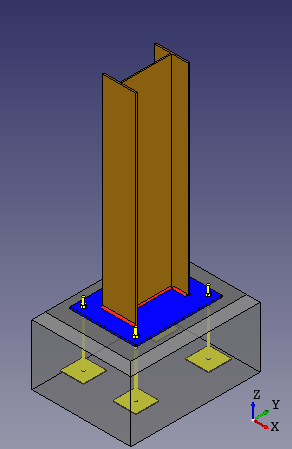
\includegraphics[width=\linewidth]{{"E:/workspace/Osdag3./ResourceFiles/images/3d}.png}%
\caption{3D View}%
\end{figure}

%
\end{document}